%%=============================================================================
%% Resultaten
%%=============================================================================

\chapter{Resultaten}%
\label{ch:resultaten}

\section{\IfLanguageName{dutch}{Brute Force Attack op WordPress Omgevingen met Beveiligingsplugins}{Brute Force Attack on WordPress enviroment with securityplugins}}
Binnen de context van webbeveiliging zijn brute force aanvallen een veelvoorkomende methode waarbij aanvallers proberen toegang te krijgen tot een systeem 
door herhaaldelijk wachtwoorden of andere inloggegevens te raden. Dit type aanval kan bijzonder schadelijk zijn voor systemen zoals WordPress, die veel 
gebruikt worden voor het bouwen van websites.In dit hoofdstuk onderzoeken we de effectiviteit van verschillende penetratietesttools bij het uitvoeren van 
brute force aanvallen op een WordPress-omgeving beveiligd met de Wordfence plugin. Het doel is niet om de beveiligingsplugins zelf te testen, maar om de 
prestaties en de mogelijkheden van de tools Burp Suite, Metasploit en OWASP ZAP met elkaar te vergelijken. Deze analyse zal helpen vaststellen welke tool 
het meest effectief en gebruiksvriendelijk is voor het tonen van kwetsbaarheden in een beschermde WordPress-omgeving.

\subsection{\IfLanguageName{dutch}{Resultaat met burp suite}{result with burp suite}}
\begin{figure}
    \centering
    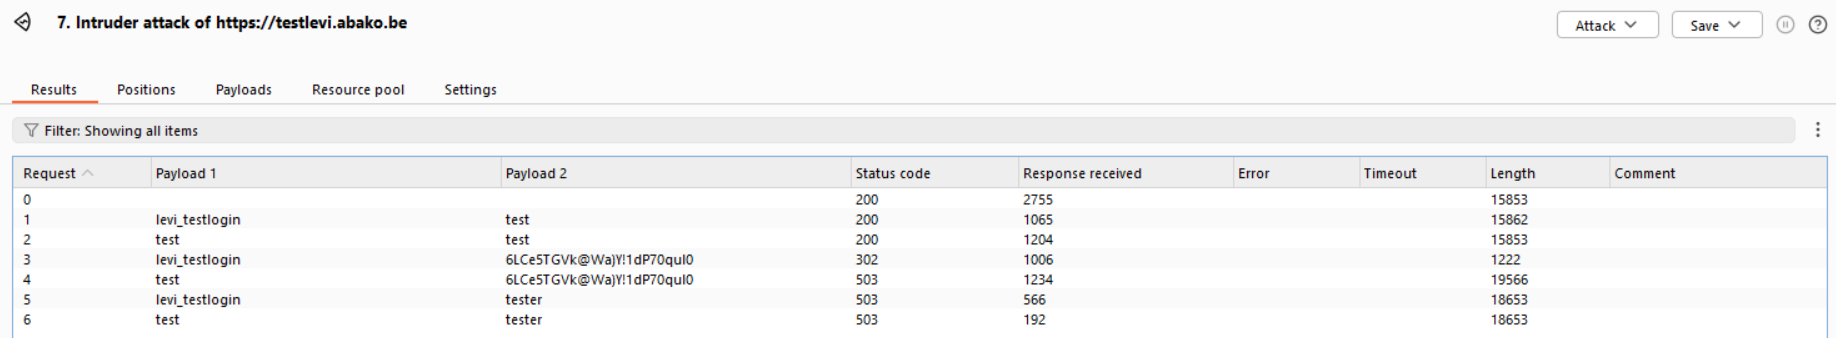
\includegraphics[height=0.1\textheight]{burp-suite_bruteforce_wordpressplugins.png}
    \caption[Burp suite brute force attack op wordpress applicatie met beveiligingsplugin]{Burp suite brute force attack op wordpress applicatie met beveiligingsplugin}
\end{figure}
De brute force attack op de WordPress omgeving met wordfence werd uitgevoerd met behulp van Burp Suite Community Edition. Tijdens de test viel het 
op dat enkele functionaliteiten beperkt waren vanwege de beperkingen van de Community Edition. Dit beperkte de mogelijkheden van het uitvoeren van een volledige 
pentest, maar het voordeel van Burp Suite is dat er veel documentatie en tutorials beschikbaar zijn op het internet, wat nuttig kan zijn bij het oplossen van 
eventuele problemen tijdens het gebruik van de tool.

\subsection{\IfLanguageName{dutch}{Resultaat met metasploit}{result with metasploit}}
\begin{figure}
    \centering
    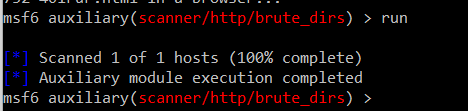
\includegraphics[height=0.1\textheight]{metasploit_brute_wordpressplugin.png}
    \caption[Metasploit brute force attack op wordpress applicatie met beveiligingsplugin]{Metasploit brute force attack op wordpress applicatie met beveiligingsplugin}
\end{figure}
Metasploit is een uiterst populair open-source framework voor beveiligingstests, dat vooral wordt ingezet voor het ontwikkelen en implementeren van exploit-codes. 
Dit framework maakt het mogelijk om systemen te evalueren op veiligheid door kwetsbaarheden actief te benutten, te identificeren 
en te verifiëren. Metasploit beschikt over honderden exploit-modules die een breed scala aan bekende kwetsbaarheden dekken, waardoor het als een essentieel 
instrument wordt gezien in de toolkit van veel cybersecurity-professionals.

In een praktische toepassing werd Metasploit gebruikt om een brute force attack uit te voeren op een WordPress-omgeving die beveiligd was met de Wordfence plugin. 
Voor deze test moest de tool via de terminal bediend worden. Hoewel dit als een beperking kan worden gezien, biedt Metasploit desondanks een uitgebreid scala aan 
mogelijkheden voor het uitvoeren van penetratietests. De tool stelt gebruikers in staat om diverse aanvalsscenario’s te simuleren en levert een uitgebreide reeks 
modules voor het uitvoeren van verschillende soorten beveiligingstests. Deze flexibiliteit en diepgang maken Metasploit een waardevolle keuze voor professionals die 
uitgebreide beveiligingstests willen uitvoeren op complexe netwerken en systemen.

\subsection{\IfLanguageName{dutch}{Resultaat met OWASP ZAP}{result with OWASP ZAP}}
\begin{figure}
    \centering
    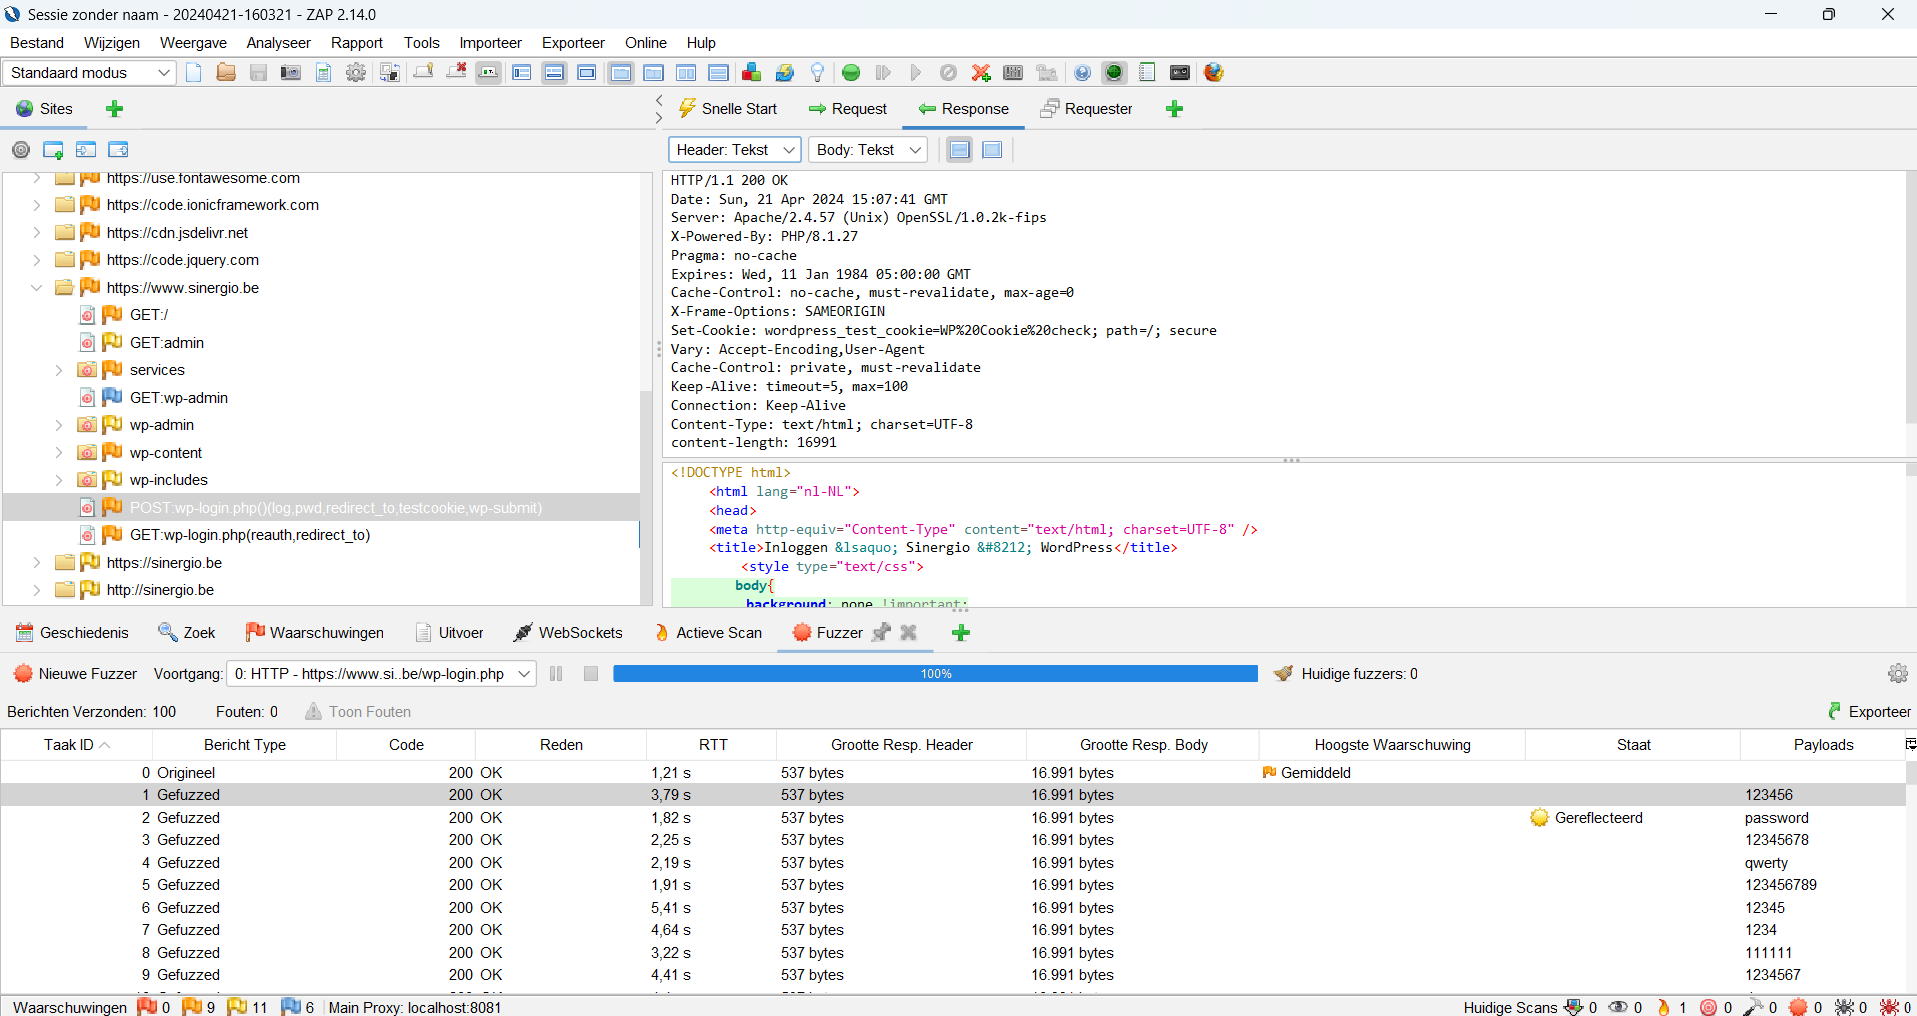
\includegraphics[height=0.3\textheight]{ZAP_brute_wordpressplugin.png}
    \caption[OWASP ZAP brute force attack op wordpress applicatie met beveiligingsplugin]{OWASP ZAP brute force attack op wordpress applicatie met beveiligingsplugin}
\end{figure}

Voor de brute force attack op de WordPress omgeving met wordfence werd OWASP ZAP gebruikt, een open source tool die bekend staat om zijn gebruiksgemak. 
Wat opviel bij het gebruik van OWASP ZAP was dat de testen vergelijkbaar konden worden uitgevoerd als bij Burp Suite, maar dan met een open source alternatief. 
Dit maakte OWASP ZAP een aantrekkelijke keuze voor organisaties die op zoek zijn naar een kosteneffectieve oplossing voor het uitvoeren van beveiligingstests.


\section{\IfLanguageName{dutch}{Vergelijking van omgevingen}{Comparison of environments}}
\begin{figure}
    \centering
    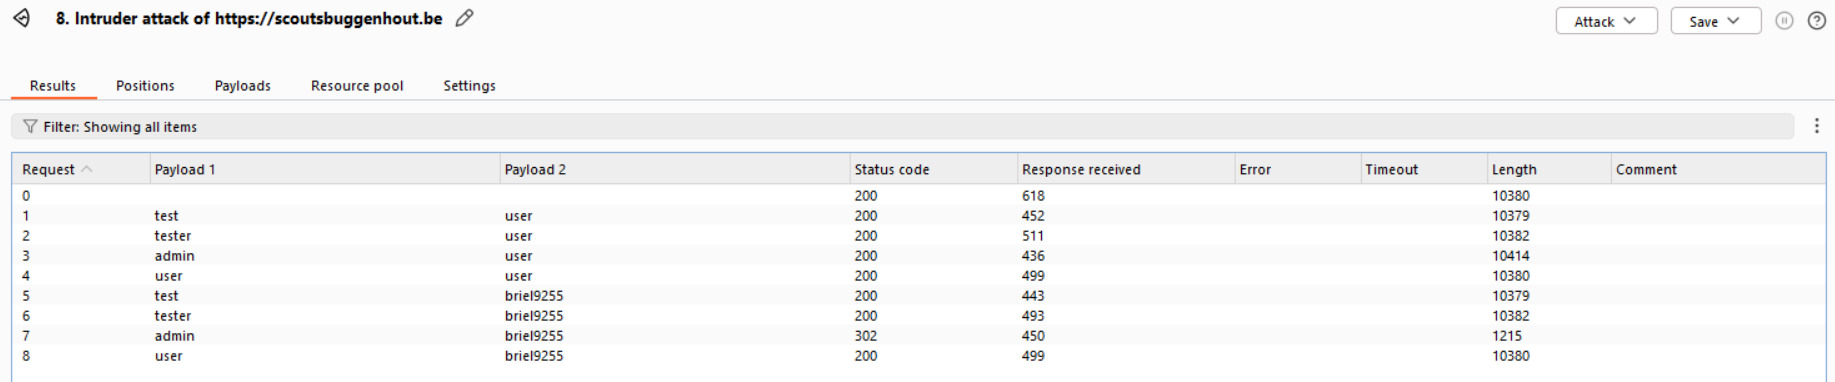
\includegraphics[height=0.1\textheight]{burp-suite_bruteforce_wordpress.png}
    \caption[Brute force aanval op een wordpress applicatie zonder beveiligingsplugins]{Brute force aanval op een wordpress site zonder beveiligingsplugins}
\end{figure}
\subsection{\IfLanguageName{dutch}{WordPress Zonder Beveiligingsplugins}{WordPress without securityplugins}}
De eerste testomgeving was een standaard WordPress-applicatie zonder enige vorm van beveiligingsplugins. De resultaten toonden aan dat deze 
omgeving bijzonder kwetsbaar was voor brute force aanvallen. Aanvallers zijn in staat om binnen enkele minuten toegang te verkrijgen door middel 
van standaard gebruikersnamen zoals 'admin' en algemeen bekende zwakke wachtwoorden. Deze bevindingen benadrukken de noodzaak voor 
basisbeveiligingsmaatregelen, zoals het instellen van sterke wachtwoorden en het gebruik van gebruikersnaam diversificatie om de initiële 
verdedigingslinie te versterken.

\begin{figure}
    \centering
    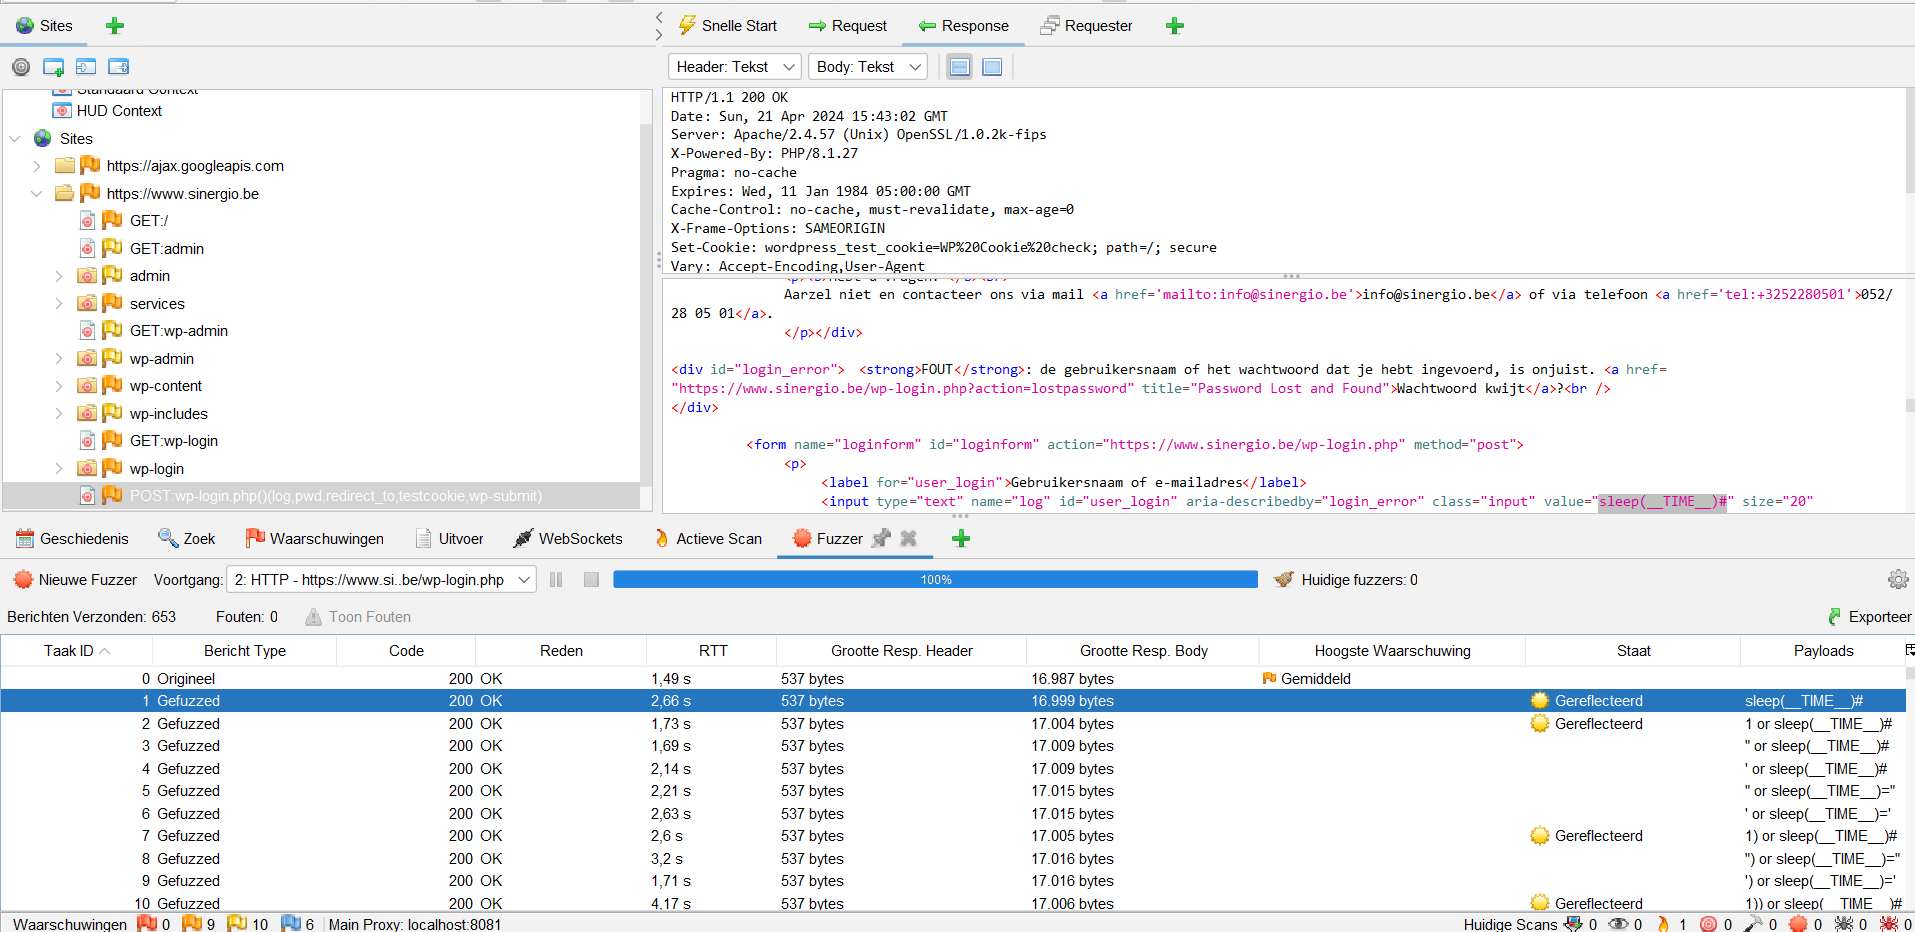
\includegraphics[height=0.2\textheight]{zap_sql-injection_wordpressplugin.png}
    \caption[SQL-injection aanval op een wordpress applicatie met beveiligingsplugins]{SQL-injection aanval op een wordpress applicatie met beveiligingsplugins}
\end{figure}
\subsection{\IfLanguageName{dutch}{WordPress Met Beveiligingsplugins}{WordPress with securityplugins}}
De tweede omgeving, een WordPress-installatie uitgerust met specifieke beveiligingsplugins, liet een aanzienlijke verbetering zien in beveiliging 
tegen brute force aanvallen. De plugins die werden getest, bieden functionaliteiten zoals limieten op inlogpogingen, directe accountvergrendeling 
bij verdachte activiteiten, en real-time monitoring en alerts. Deze maatregelen leidden tot een snelle detectie en blokkering van aanvalspogingen, 
waardoor de veiligheid van de omgeving aanzienlijk werd verhoogd. Deze resultaten onderstrepen het belang van het toepassen van gespecialiseerde 
beveiligingsuitbreidingen in populaire CMS-systemen, wat aantoont dat zelfs basale beveiligingsplugins een significante bescherming kunnen bieden.

\begin{figure}
    \centering
    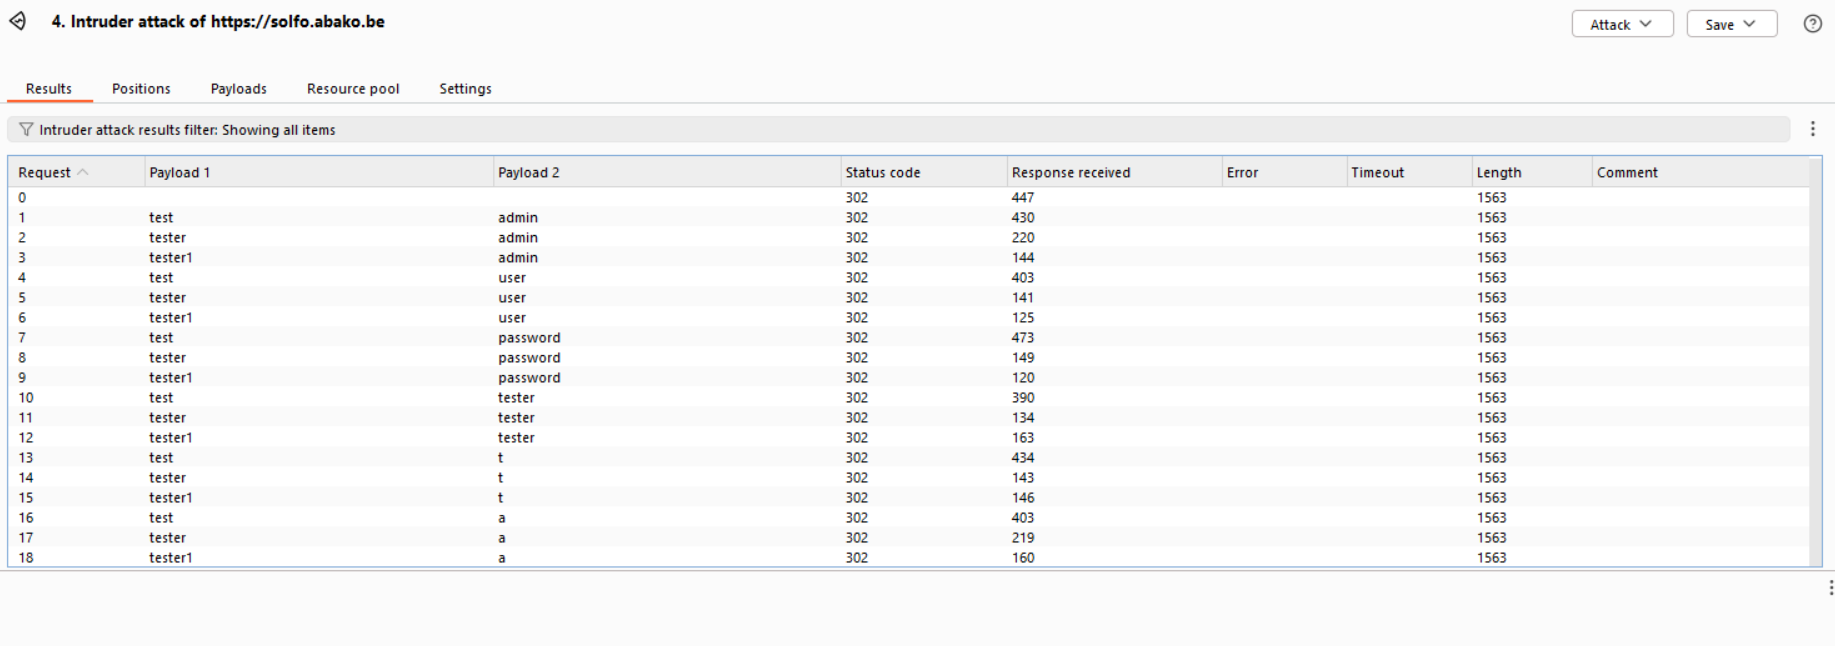
\includegraphics[height=0.2\textheight]{burp-suite_bruteforce_laravel.png}
    \caption[Brute force aanval op een laravel applicatie]{Brute force aanval op een laravel applicatie}
\end{figure}
\subsection{\IfLanguageName{dutch}{Laravel Applicatie}{Laravel Application}}
De Laravel-applicatie, bekend om zijn robuuste beveiligingsarchitectuur, vertoonde uitmuntende prestaties tijdens de brute force test. De 
ingebouwde beveiligingsmaatregelen van Laravel, zoals geavanceerde gebruikersauthenticatie en automatische beveiliging tegen veelvoorkomende 
kwetsbaarheden, boden een solide bescherming. De applicatie was niet alleen bestand tegen brute force pogingen, maar implementeerde ook 
standaard versleutelingstechnieken die de integriteit en vertrouwelijkheid van gebruikersgegevens garanderen. Deze bevindingen illustreren 
hoe een framework met ingebouwde beveiliging kan dienen als een effectieve basis voor het ontwikkelen van veilige webapplicaties.
